\documentclass[letterpaper, reqno,11pt]{article}
\usepackage[margin=1.0in]{geometry}
\usepackage{color,latexsym,amsmath,amssymb,graphicx,float,listings,tikz}
\usepackage{hyperref}

\hypersetup{
colorlinks=true,
linkcolor=magenta,
filecolor=magenta,
urlcolor=cyan,
}

\graphicspath{ {images/} }

\begin{document}
\pagenumbering{arabic}
\title{Math 318 Homework 9}
\date{31/03/23}
\author{Xander Naumenko}
\maketitle

{\medskip\noindent\bf Question 1a.} Any states that involve more than one book to the front can never happen, and otherwise the probability is just $\frac{1}{6}$ if the new front is B/C and $\frac{2}{3}$ if $A$ is (I wrote the matrix backwards originally so note the transpose):
\[
    P=\begin{pmatrix}
        \frac{2}{3}&0&\frac{2}{3}&\frac{2}{3}&0&0\\
        0&\frac{2}{3}&0&0&\frac{2}{3}&\frac{2}{3}\\
        \frac{1}{6}&\frac{1}{6}&\frac{1}{6}&0&0&0\\
        0&0&0&\frac{1}{6}&\frac{1}{6}&\frac{1}{6}\\
        \frac{1}{6}&\frac{1}{6}&0&0&\frac{1}{6}&0\\
        0&0&\frac{1}{6}&\frac{1}{6}&0&\frac{1}{6}
    \end{pmatrix}^T
.\]

{\medskip\noindent\bf Question 1b.} In the stationary distribution we have that $P\pi=\pi \implies (P-I)\pi=0$, i.e.
\[
    \begin{pmatrix}x_1\\x_2\\x_3\\x_4\\x_5\\x_6\end{pmatrix}^T
    \begin{pmatrix}
        -\frac{1}{3}&0&\frac{2}{3}&\frac{2}{3}&0&0\\
        0&-\frac{1}{3}&0&0&\frac{2}{3}&\frac{2}{3}\\
        \frac{1}{6}&\frac{1}{6}&-\frac{5}{6}&0&0&0\\
        0&0&0&-\frac{5}{6}&\frac{1}{6}&\frac{1}{6}\\
        \frac{1}{6}&\frac{1}{6}&0&0&-\frac{5}{6}&0\\
        0&0&\frac{1}{6}&\frac{1}{6}&0&-\frac{5}{6}
        \end{pmatrix}^T=0
\]
\[
    \begin{pmatrix}
        -\frac{1}{3}&0&\frac{2}{3}&\frac{2}{3}&0&0\\
        0&-\frac{1}{3}&0&0&\frac{2}{3}&\frac{2}{3}\\
        \frac{1}{6}&\frac{1}{6}&-\frac{5}{6}&0&0&0\\
        0&0&0&-\frac{5}{6}&\frac{1}{6}&\frac{1}{6}\\
        \frac{1}{6}&\frac{1}{6}&0&0&-\frac{5}{6}&0\\
        0&0&\frac{1}{6}&\frac{1}{6}&0&-\frac{5}{6}
        \end{pmatrix}
    \begin{pmatrix}x_1\\x_2\\x_3\\x_4\\x_5\\x_6\end{pmatrix} =0
\]
\[
\implies \pi=\begin{pmatrix} 10\\10\\4\\1\\4\\1 \end{pmatrix} \frac{1}{30}
.\]

{\medskip\noindent\bf Question 1c.} The state BCA is $i=4$. As we proved in class then the expect number of steps to return is $\frac{1}{\pi_i}=30$.

{\medskip\noindent\bf Question 2a.} If it doesn't rain then $X_{n+1}=4-X_{n}$. If it does rain, then if $n\neq 1$ then $X_{n+1}=5-X_n$. Thus the transition matrix, with the indices being $0,1,2,3,4$ is
\[
\begin{pmatrix} 
    0&0&0&0&1\\
    0&0&0&1-p&p\\
    0&0&1-p&p&0\\
    0&1-p&p&0&0\\
    1-p&p&0&0&0
\end{pmatrix} 
.\]

{\medskip\noindent\bf Question 2b.} Finding the stationary distribution, we first find an eigen vector by setting $\pi_4=1$ and solving the equation $\pi(P-I)=0$ then scaling to be a proper probability vector:
\[
\implies v=\begin{pmatrix} 1-p\\ 1\\ 1\\ 1\\ 1 \end{pmatrix}\frac{1}{5-p}
.\]
We can now verify that $\pi_i P_{ij}=\pi_j P_{ji}$. Checking this for each $i,j\in [4]$, this confirms that the chain is reversible.

{\medskip\noindent\bf Question 2c.} The only way that he gets wet is if both he is in state $\pi_0$ and the $p$ chance that it rains occurs. In the stationary distribution being in $\pi_0$ is $\frac{1-p}{5-p}$, so the probability that he's wet on a given trip is $\frac{p(1-p)}{5-p}$.

{\medskip\noindent\bf Question 2d.} To maximize this probability you can take the derivative and set it to 0: 
\[
\frac{d}{dp}\frac{p(1-p)}{5-p}=0\implies p^2-10p+5=0\implies p=5-2\sqrt{5} 
.\]
This is greater than the value at the boundary ($p=0,p=1$), so it is the maximum.

{\medskip\noindent\bf Question 2e.} The transition probability would be the same as part a in the same pattern (i.e. diagonal going upwards with $p$ then $1-p$), just extended to a larger $N$. Therefore the stationary state would be
\[
\pi= \begin{pmatrix} 1\\1\\ \vdots \\ 1\\ \frac{1}{1-p}\end{pmatrix}\frac{1}{N+1-p}
.\]
The probability that he gets wets on a given day is then $\frac{p(1-p)}{N+1-p}$, and to find the $p$ that maximizes this probability would be the solution to the problem $\frac{d}{dp}\left( \frac{p(1-p)}{N+1-p} \right) $ (given the question is quite vague I assume I don't have to actually solve this).

{\medskip\noindent\bf Question 3.} Same as question 2.

{\medskip\noindent\bf Question 4.} As the hint suggests, consider $q$ to be the probability of ever getting to $n-1$ starting on $n$. This is independent on $n$, as the probability transitions are also independent of $n$. From a given $n$, there are two ways to go to $n-1$: either directly there with probability $1-p$, or go up once with probability $p$ and eventually make it back to $n$ then $n-1$, which happens with probability $q^2$. Thus
\[
    q=1-p + pq^2\implies pq^2-q+1-p=0 \implies q=\frac{1}{p}-1\text{ or }
.\]
Note that if $p<\frac{1}{2}$ then the formulation above isn't valid since $q=1$ (since the random walk is then recurrent). Thus if $p>\frac{1}{2}$ then $q=\frac{1}{p}-1$, and $q=1$ otherwise.

Now for the actual problem, note that if the first state that is taken is downward then we are guaranteed to return to 0 since $p>\frac{1}{2}$, and otherwise the probability to return is $q$. Thus we have
\[
P=1-p+pq=1-p+p(\frac{1}{p}-1)=2-2p
.\]

{\medskip\noindent\bf Question 5.} Consider this random walk as a walk on graph with $52!$ nodes, each node denoting a particular permutation of the cards. Two nodes are connected if they are identical except one node flipped. Each node has $52\cdot 51$ neighbors (number of choices of 2 distinct neighbors). For the uniform distribution $\pi$ over all possible states, for each state $i$ we have $\pi_i=\frac{1}{52!}$. The next state is given by
\[
    \pi_{i}P_i=52\cdot 51 \frac{1}{52! 52\cdot 51}=\frac{1}{52!}
.\]
Since $\pi_iP_i=\pi_{i}$ for all $i$, the uniform distribution $\pi_i$ is the stationary distribution.

{\medskip\noindent\bf Question 6a.} See figure \ref{fig:q6} for the graph.  The code is as follows:

\begin{lstlisting}
import random
import matplotlib.pyplot as plt

F_n = []
n = 1000
for s in range(n):
    cards = list(range(52))
    F_n.append([52])
    for _ in range(200):
        i = random.randint(0, 51);
        j = random.randint(0, 51);
        temp = cards[i]
        cards[i] = cards[j]
        cards[j] = temp

        f_n = F_n[-1][-1]
        if cards[i] == j:
            f_n-=1
        if cards[j] == i:
            f_n-=1
        if cards[i] == i:
            f_n+=1
        if cards[j] == j:
            f_n+=1
        F_n[-1].append(f_n)

F_n_avg = [sum([f[i] for f in F_n]) / n for i in range(len(F_n[0]))]
print(F_n_avg)

plt.plot(F_n_avg);

plt.show()
\end{lstlisting}

{\medskip\noindent\bf Question 6b.} As confirmed with the code, the expected value of $F$ in the stationary state is $F=1$. Given that this is a simulation question I don't think I have to justify my answer, but intuitively at least it's because the stationary state is randomly shuffled, and in this state each card has a $\frac{1}{52}$ chance of being in its correct place (although properly proving that you can sum these is more complicated since they're not independent).

\begin{figure}[htpb]
    \centering
    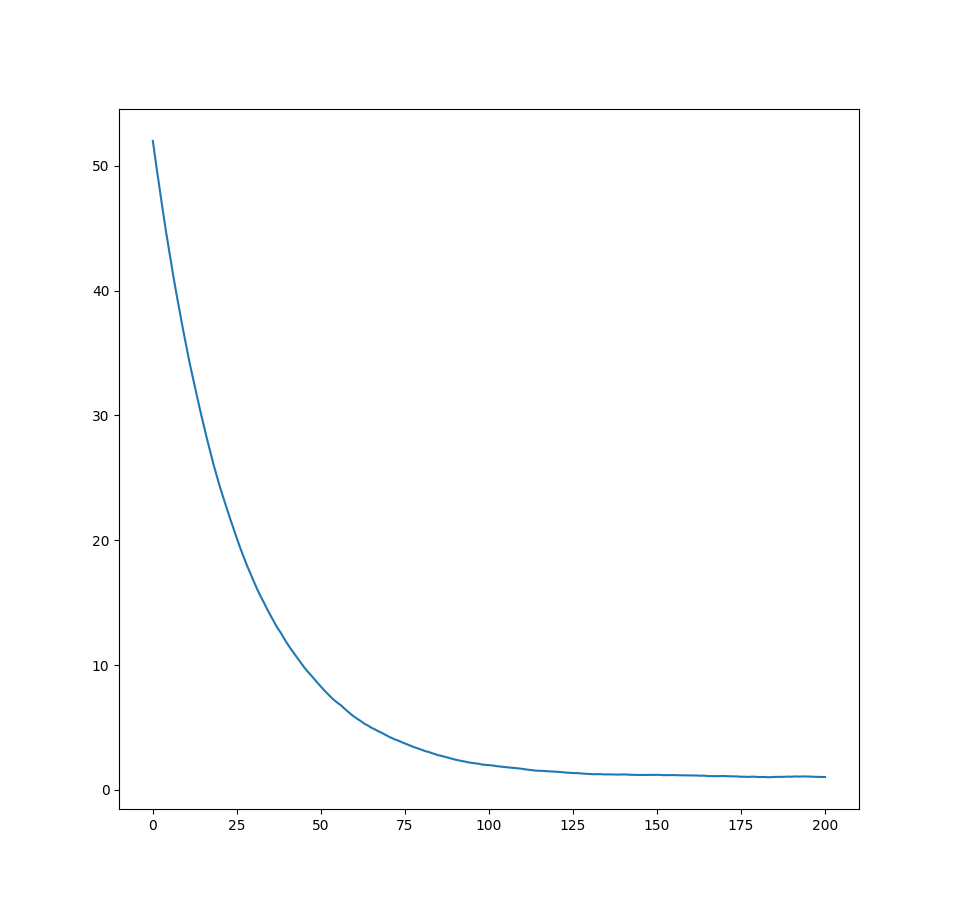
\includegraphics[width=0.8\textwidth]{q6}
    \caption{Graph for question 6}
    \label{fig:q6}
\end{figure}

\end{document}
